\documentclass[sigconf,anonymous,review]{acmart}
\setcopyright{none}
\setlength{\emergencystretch}{2em}
\settopmatter{printacmref=false}
\renewcommand\footnotetextcopyrightpermission[1]{}
\acmConference{}{}{}
\acmYear{2026}
\title{Certifying Reward Alignment in Portfolio Reinforcement Learning}
\author{Anonymous Author(s)}
\newcommand{\E}{\mathbb{E}}
\newcommand{\Var}{\operatorname{Var}}
\newcommand{\Cov}{\operatorname{Cov}}
\newcommand{\spn}{\operatorname{span}}
\newcommand{\eq}{\mathrm{eq}}
\newtheorem{proposition}{Proposition}
\newtheorem{theorem}{Theorem}
% Generated from all final saved policies.
\newcommand{\NSeeds}{20}
\newcommand{\MyopicD}{0.610183}
\newcommand{\OrdinaryD}{0.250692}
\newcommand{\CentredD}{0.249259}
\newcommand{\MyopicE}{0.003198}
\newcommand{\OrdinaryE}{0.000606}
\newcommand{\CentredE}{0.000594}
\newcommand{\DistanceReduction}{59.2}
\newcommand{\DeviationReduction}{81.4}
\newcommand{\CentreReduction}{0.57}
\newcommand{\PpoText}{With PPO, the continuation correction reduces mean distance by 33.3\% and maximum deviation gain by 49.8\%. The paired distance difference is -0.575 (95\% seed-bootstrap interval [-0.739, -0.404]).}

\begin{document}
\begin{abstract}
A portfolio agent can optimise its reward accurately while implementing a different financial preference. We develop an audit that connects a learned policy to a specified terminal mean--variance equilibrium. In a finite exogenous-state market, we bound the gain from changing one decision by actor, reward and continuation-critic errors. The bound is invariant to state-constant critic offsets, extends to convex action constraints, and admits an independent-sample version that does not require the equilibrium policy. A continuation-aware actor--critic implementation replaces the oracle used by exact reward calibration. Across nine controlled markets and twenty seeds, it reduces policy distance by \DistanceReduction\% relative to a matched myopic-reward network; a separate PPO experiment tests the reward intervention with a standard policy optimiser. Historical allocation tests cross six covariance estimators and 10, 30 and 49 US industry portfolios over 432 months. They show that preserving a fitted mandate differs from improving realised investment performance. The contribution is an inspectable link between reward design, finite-budget learning and financial decisions, with policy alignment evaluated separately from investment performance.
\end{abstract}
\ccsdesc[500]{Computing methodologies~Reinforcement learning}
\ccsdesc[300]{Applied computing~Economics}
\keywords{financial reinforcement learning, reward alignment, equilibrium, actor--critic, model validation}
\maketitle

\section{Introduction}
An investment mandate specifies a preference over return, risk and costs. A reinforcement-learning agent receives a reward and learns a policy. These descriptions need not imply the same decisions. Replacing variance by a second moment penalises squared expected return as well as risk; ignoring dependence removes a hedge against future opportunities; correcting risk while leaving costs unchanged can alter the effective turnover preference. A favourable backtest does not establish that these changes preserve the mandate.

Kolm and Ritter~\cite{kolm2025}, pp.~90--91, identify reward design and mandate alignment as practical concerns. Their workflow places reward specification before agent training. We make the connection between those stages testable: first audit what the reward implements, then audit what the trained agent implements. When an exact target is available, this means comparing policies under common information and constraints. When it is unavailable, we ask how much the investor could improve the intended objective by changing one decision while retaining the agent's future policy.

This distinction matters for actor--critic learning. A zero actor gradient need not indicate a financial equilibrium if the continuation critic is wrong. Conversely, a large critic value error can be irrelevant to decisions if it is a constant across states. We derive a residual certificate that distinguishes these cases. Its critic term uses state differences and their propagation through the market dynamics, rather than absolute value error alone. The result supplies a stopping or rejection criterion under explicit model and data assumptions.

The audit also separates reward errors from estimation risk. Markowitz~\cite{markowitz1952} distinguishes beliefs about returns from decisions made using them. DeMiguel et al.~\cite{demiguel2009} show that estimation error can overwhelm gains from optimal diversification. We therefore retain a historical factorial experiment in which covariance models and rewards are changed separately. Correctly implementing estimated opportunities is not the same as estimating them correctly.

Our contributions are a finite-iterate deviation certificate for terminal mean--variance equilibrium; a sample-based implementation and controlled neural/PPO comparisons; and a historical audit that separates covariance, reward and numerical effects. The backward learner builds on existing equilibrium RL, the calibration uses an established mean auxiliary, and the confidence bounds use standard concentration results. The new focus is the quantitative connection from these components to the financial decision made by a trained agent.

\section{Related work}
\paragraph{Financial objectives and estimation.}
DeMiguel, Garlappi and Uppal~\cite{demiguel2009}, Tables~3--5, compare fourteen allocation models with $1/N $. Their Proposition~1 and Figure~1 explain estimation requirements as a function of dimension and investment opportunities; they do not prescribe a minimum number of assets. Their Table~2 includes ten industries plus the market. We retain a compact industry benchmark and test finer classifications. Linear shrinkage~\cite{ledoit2004identity,ledoit2004correlation}, nonlinear shrinkage~\cite{ledoit2017} and observed-factor covariance~\cite{fan2008} address the input side of this problem. We implement the two linear estimators and factor models, not nonlinear shrinkage.

G\^arleanu and Pedersen~\cite{garleanu2013}, Eq.~(4) and Propositions~2--3, derive cost-aware dynamic allocation; DeMiguel et al.~\cite{demiguel2024}, Eq.~(6) and Tables~II--III, study conditional multifactor portfolios with costs. These are positive examples of explicit financial preferences. Our rolling one-period L1-cost reference is a different object. Neither a change in covariance estimator nor an intentional change in preference should be called reward misspecification.

\paragraph{Financial RL and reward design.}
Kolm and Ritter's earlier hedging work~\cite{kolm2019}, Eqs.~(8)--(10), explicitly treats quadratic increment rewards as an approximation. Jiang et al.~\cite{jiang2025}, Eq.~(8), combine log return and variance; their 2024 formulation~\cite{jiang2024}, Eq.~(4), also considers costs. Habibnia and Soltanzadeh~\cite{habibnia2024}, Eq.~(8), use asymmetric PnL with SAC, shorting and lending. Table~\ref{tab:historical} adapts reward formulations to common states; it does not reproduce these papers' complete agents or backtests.

Objective-aware learning is established. The reward in Simon et al.~\cite{simon2026}, Eq.~(17), is centred mean--variance utility. Gollart and Okhrin~\cite{gollart2025}, Section~4.2.1, compare learned policies with an analytical benchmark. Cong et al.~\cite{cong2026}, Eqs.~(19)--(20), permit differentiable trajectory objectives. Kolm and Ritter's 2025 article is an overview, not a new numerical baseline. Its discussion of known-policy validation (p.~87) precludes claiming that benchmark comparison itself is new.

\paragraph{Equilibrium learning and certification.}
Precommitment~\cite{ling2000} and equilibrium~\cite{basak2010} solve different decision problems. Continuation hedges~\cite{czichowsky2013}, equivalent objectives~\cite{bkm2016} and equilibrium RL~\cite{dai2023} precede our work. Lesmana and Pun~\cite{lesmana2025} develop subgame-perfect equilibrium RL and backward policy iteration; our implementation specialises these principles. We use their 2021 preprint for algorithm details; we do not replicate the final 2025 implementation. Guo et al.~\cite{guo2026}, Algorithms~1--3, already combine auxiliary rewards, deterministic policy gradients and fixed-point critic learning. We do not propose a new general equilibrium solver.

Sangadi et al.~\cite{sangadi2025}, Theorem~4.3, provide finite-sample actor--critic stationarity analysis for a discounted return mean--variance objective. Our target is instead a posteriori, statewise one-step deviation gain for a given finite-horizon policy. Seminorm learning and irrelevant critic offsets are also established~\cite{chen2025seminorm}. We use that geometry to obtain a financial error certificate. The scalar reward-calibration identity below follows the mean auxiliary in MVPI~\cite{zhang2021}; the empirical Bernstein allowance follows Maurer and Pontil~\cite{maurer2009}. The contribution lies in the resulting decision audit, not in inventing these ingredients.

\section{Objectives and reward calibration}
\subsection{Terminal and fitted references}
Let $Z_t $ be a finite exogenous Markov state and let excess returns $R_t\in\mathbb R^d $ be jointly distributed with $Z_{t+1}$ conditional on $Z_t $. Wealth obeys
\begin{equation}\label{eq:wealth}
 X_{t+1}=sX_t+R_t^\top u_t(Z_t),\qquad H_t=s^{T-t-1},
\end{equation}
where $s>0$ is deterministic. The financial criterion at each state is conditional terminal mean minus $\varphi>0$ times terminal variance. We consider deterministic wealth-independent policies and their one-step deviations, holding future policies fixed. This equilibrium criterion differs from maximising initial-date precommitment value.

For independent returns with mean $m_t $ and covariance $\Sigma_t\succ0$, equilibrium is $u_t^\eq=\Sigma_t^{-1}m_t/(2\varphi H_t)$. With $M_t=\Sigma_t+m_tm_t^\top $ and $\nu_t=m_t^\top M_t^{-1}m_t $, the additive reward
\begin{equation}\label{eq:independent}
 Y_t-\varphi(1-\nu_t)Y_t^2,\qquad Y_t=H_tR_t^\top u_t,
\end{equation}
recovers that policy. This specialises prior equivalent-objective constructions~\cite{bkm2016}. Under dependence, continuation covariance is essential; Eq.~\eqref{eq:independent} alone is insufficient.

For the raw family $\Delta X-\kappa(\Delta X)^2$, even optimal constant scalar tuning leaves a discrepancy. With independent constant moments and $m\ne0$, $d=M^{-1}m $, $\nu=m^\top d $, $b=[2\varphi(1-\nu)]^{-1}$ and fixed $T\ge2$,
\begin{align}\label{eq:raw}
\min_{\kappa>0}D&=c_T|s-1|+O((s-1)^2),\\
c_T&=\|d\|b\sqrt{\tfrac{T(T^2-1)}3+\tfrac{\nu(1-\nu)T(T-1)}2}.\nonumber
\end{align}
Here $D^2=\sum_t\E_{\pi^\kappa}\|\pi^\kappa(t,X_t)-u_t^\eq\|^2$ uses the raw-reward optimum's occupancy. Appendix~\ref{app:raw} supplies the derivation. This obstruction concerns one reward family, not all additive rewards.

\subsection{Constraints and deterministic costs}
For historical data we use a separate, fitted one-period target
\begin{equation}\label{eq:fitted}
 F(u)=m^\top u-\varphi u^\top\Sigma u-g(u),\quad u\in C,
\end{equation}
where $C $ is the simplex and $g(u)=\lambda\|u-p\|_1$ at pre-trade holdings $p $. Its optimum $u^*$ is not the true historical market optimum. For $a=m^\top u^*$ and $A=1+2\varphi a>0$, define
\begin{equation}
 Q_a(u)=m^\top u-\frac{\varphi}{A}u^\top Mu-\frac{g(u)}A.
\end{equation}
The identity
\begin{equation}\label{eq:aux}
 A Q_a(u)=F(u)-\varphi(m^\top u-a)^2+\varphi a^2
\end{equation}
proves that both objectives have the same maximiser. It is an application of the MVPI auxiliary~\cite{zhang2021}, not a new general algorithm. Correcting risk alone introduces the extra term $-2\varphi a\,g(u)$ and can change the cost preference.

For any anchor $a $ with $A>0$, an $\epsilon $-optimal $\widehat u $ for $Q_a $ satisfies
\begin{equation}\label{eq:anchor}
 F(u^*)-F(\widehat u)\le\varphi(m^\top u^*-a)^2+A\epsilon.
\end{equation}
This follows by comparing Eq.~\eqref{eq:aux} at $u^*$ and $\widehat u $. For convex $C,g $ and $\Sigma\succ0$, divide by $\varphi\lambda_{\min}(\Sigma)$ to bound squared allocation distance. The result includes deterministic borrowing and shorting charges, provided all costs are scaled. Choosing $a=m^\top p $ gives one existing MVPI update without supplying $u^*$; it is approximate rather than an exact calibration certificate.

\section{Certifying a learned equilibrium}
\subsection{A decision-relevant critic error}
Assume finite second moments, $\Sigma_t(z)\succ0$, and that future innovations are conditionally independent of $R_t $ given $Z_{t+1}$. Let $P_t $ denote the exogenous transition matrix. For a candidate policy $u $, the expected remaining terminal excess gain satisfies
\begin{equation}\label{eq:a}
 a_T=0,\qquad a_t=H_tm_t^\top u_t+P_ta_{t+1}.
\end{equation}
A one-step deviation to $v $ changes the terminal criterion through
\begin{equation}\label{eq:local}
 J_t(v)=H_tm_t^\top v-\varphi H_t^2v^\top\Sigma_tv
 -2\varphi H_t\Cov_t(R_t,a_{t+1}(Z'))^\top v+\mathrm{const}.
\end{equation}
The conditional independence and wealth-independent continuation assumptions justify the covariance reduction. They do not hold for arbitrary latent-state trading policies.

For any critic $c_t(z)$, define residuals and a critic-based action gradient by
\begin{align}
 e_t&=c_t-H_tm_t^\top u_t-P_tc_{t+1},\label{eq:residual}\\
 g_t&=H_tm_t-2\varphi H_t\Cov_t(R_t,c_{t+1}(Z'))
       -2\varphi H_t^2\Sigma_tu_t.\label{eq:gradient}
\end{align}
Use $\spn(f)=\max_z f(z)-\min_z f(z)$ and the Dobrushin coefficient
$\rho_t=\frac12\max_{z,w}\sum_j|P_t(z,j)-P_t(w,j)|$. Set
\begin{equation}\label{eq:span}
 S_T=\spn(c_T),\qquad S_t=\spn(e_t)+\rho_tS_{t+1}.
\end{equation}
No equilibrium policy appears in these quantities.

\begin{theorem}\label{th:audit}
Let $\mathcal E_t(z)=\sup_v[J_t(v)-J_t(u_t(z))]$. Under the preceding assumptions, with unrestricted deviations,
\begin{equation}\label{eq:audit}
 \sqrt{\mathcal E_t(z)}\le
 \frac{\|g_t(z)\|_{\Sigma_t(z)^{-1}}}{2\sqrt\varphi H_t}
 +\frac{\sqrt\varphi}{2}S_{t+1}.
\end{equation}
For a feasible policy on a fixed nonempty closed convex action set, replace the first term by $\sqrt{\mathcal E_t^c(z)}$, the maximal feasible improvement in Eq.~\eqref{eq:local} with $a_{t+1}$ replaced by $c_{t+1}$, assuming its maximum is attained. The same bound holds.
\end{theorem}
\begin{proof}
Write $\delta=c-a $. Equations~\eqref{eq:a}--\eqref{eq:residual} give $\delta_t=e_t+P_t\delta_{t+1}$. Stochastic-kernel span contraction implies $\spn(\delta_t)\le S_t $. The true action gradient is $d_t=g_t+2\varphi H_t\Cov_t(R_t,\delta_{t+1})$. Completing the square yields
$\mathcal E_t=\|d_t\|_{\Sigma_t^{-1}}^2/(4\varphi H_t^2)$.
For any scalar $D $, linear-projection residual variance is nonnegative, so
\[
\|\Cov(R,D)\|_{\Sigma^{-1}}^2\le\Var(D)\le\spn(D)^2/4.
\]
The triangle inequality proves Eq.~\eqref{eq:audit}.

For constraints, write $J=J_c+b^\top v+\mathrm{const}$, $b=2\varphi H\Cov(R,\delta)$ and $k=\varphi H^2$. If $v_c $ maximises $J_c $, strong concavity and its variational inequality imply
$J_c(v)-J_c(v_c)\le-k\|v-v_c\|_\Sigma^2$ and
$\|v_c-u\|_\Sigma\le\sqrt{\mathcal E^c/k}$. Thus
\[
 \mathcal E\le\mathcal E^c+\|b\|_{\Sigma^{-1}}\sqrt{\mathcal E^c/k}
       +\frac{\|b\|_{\Sigma^{-1}}^2}{4k}
 =\left(\sqrt{\mathcal E^c}+\frac{\|b\|_{\Sigma^{-1}}}{2\sqrt k}\right)^2.
\]
Apply the preceding covariance bound.
\end{proof}
The maximum certified $\mathcal E_t(z)$ bounds a one-step equilibrium deviation, not global-policy regret. Adding arbitrary time-dependent state-constant offsets to $c $ leaves the certificate unchanged. If $\rho_t\le\rho<1$ and residual spans are at most $\eta $, the critic contribution depends on a geometric sum, rather than an unweighted horizon sum. This uses established seminorm geometry~\cite{chen2025seminorm}. The vector result has no explicit dimension factor in the critic term; reliable covariance estimation remains dimension-dependent.

\subsection{Reward error, actor error and sampled audits}
If a learner follows a different action gradient $h_t $, split $g_t=h_t+(g_t-h_t)$ in Eq.~\eqref{eq:audit}. This gives nonnegative actor, reward and critic terms, respectively. It is an upper bound, not an additive decomposition of realised returns. A small neural parameter gradient is insufficient: a saturated actor may have a small parameter derivative despite a large action gradient. At a constraint boundary, use the feasible improvement in Theorem~\ref{th:audit} rather than an unconstrained gradient norm.

The exact-model certificate uses conditional moments. For scalar bounded returns, a separate independent-data construction estimates its gradient, variance and Bellman residuals using confidence bounds (Appendix~\ref{app:data}). It conditions on a policy and critic fixed before the audit and does not use the equilibrium policy. If the variance lower bound is nonpositive, it returns an uninformative infinite bound. These conditions rule out silently applying the guarantee to reused training data or a dependent historical time series.

\section{Learning and evaluation protocol}
\subsection{Continuation-aware sample learning}
Two independent conditional observations $(R_1,Z'_1),(R_2,Z'_2)$ yield the reward
\begin{equation}\label{eq:paired}
 L_c(v)=\frac{H(R_1+R_2)^\top v}{2}
 -\frac\varphi2\left[H(R_1-R_2)^\top v+c(Z'_1)-c(Z'_2)\right]^2.
\end{equation}
Its expected action gradient equals Eq.~\eqref{eq:gradient}. A backward mean critic learns from targets $HR^\top u+c(Z')$. This replaces oracle continuation by sampled policy evaluation, using established backward equilibrium-learning principles~\cite{lesmana2025}. Paired covariance estimation itself is standard.

Our controlled market has two observed regimes, transition probabilities $(p,1-p)$ and $(1-p,p)$, conditional edge means
\[
 \begin{pmatrix}.09&-.05\\.04&-.02\end{pmatrix},
\]
and independent innovations $\pm.12$ with equal probabilities. We set $s=1.02$, $\varphi=1$, $X_0=1$, $p\in\{.5,.8,.95\}$ and $T\in\{4,12,24\}$. Even $p=.5$ is not an iid-return experiment: returns remain jointly related to successor regimes. Exact moments and equilibrium are restricted to evaluation.

The tabular study uses 128/512/2,048/8,192 conditional samples per time/state, twenty seeds and three methods: myopic paired variance, continuation-aware actor updates, and exact optimisation of the same sampled actor objective. Its 2,160 records separate sampling from numerical optimisation. Forty actor steps use a quarter of the estimated inverse curvature; no zero variance is silently regularised.

The neural study uses 2,048 conditional samples per time/state, shared actor and critic networks with two 32-unit tanh layers, and inputs consisting of normalised time and regime one-hot encoding. Adam uses learning rate .003, target-critic averaging .02 and batch size 64 per time/state. We retain checkpoints at 250, 1,000 and 3,000 updates. The three variants use myopic reward, continuation-aware reward with an ordinary mean critic, or continuation-aware reward with state-centred critic outputs and TD targets. Hyperparameters were fixed before the five-seed pilot and retained when extending to twenty seeds. All methods share samples and initialisations. Actor losses use the same frozen, sample-estimated inverse-curvature scaling. Actions do not affect the market, and all sampled returns are observed; this generative-data setting is stronger than a single historical trajectory.

\subsection{A standard policy-optimisation comparison}
We additionally use clipped PPO~\cite{schulman2017}, Eq.~(7), via Stable-Baselines3 2.9.0. The two arms differ only in whether Eq.~\eqref{eq:paired} includes continuation covariance. Both use sample-only backward evaluation of the current deterministic policy, refreshed between rollouts; no exact equilibrium enters training. This is a structured PPO hybrid, not a reproduction of a published financial agent or a claim that PPO itself solves time inconsistency.

The protocol fixes $T=12$, $p=.8/.95$, seeds 0--9, 32,768 environment steps, actions in $[-3,3]$, and the same 2,048-sample conditional datasets. Each environment step draws a pair; the first successor advances the episode. Eight environments supply 512 observations per rollout, with ten epochs, batch size 128, learning rate $3\times10^{-4}$, clipping threshold .2, GAE parameter .95, discount 1, entropy coefficient 0, and separate 64-by-64 tanh actor/value networks. We evaluate the clipped deterministic deployment policy. Budgets are matched within PPO, not between PPO and direct-gradient learning.

\subsection{Historical allocation and common metrics}
Kenneth French's value-weighted industry returns and factors~\cite{french}, archived August 2026 vintage, provide 432 evaluation months from January 1990 to December 2025. The lagged window is 120 months; means are unshrunk excess-return means, $\varphi=5$ and L1-cost coefficient $\lambda=.001$. The data are revised research portfolios, not point-in-time investable funds. This experiment audits Eq.~\eqref{eq:fitted}; it is not a backtest of the new regime-based RL learners.

Six covariance models---sample, fixed 10\% diagonal shrinkage, Ledoit--Wolf identity and constant correlation, market factor and three Fama--French factors---are crossed with 10/30/49 industries. Within each model, rewards share target pre-trade holdings, moments and constraints. Cross-model comparisons use the diagonal-model target's holdings. Own-state paths determine realised performance. These controls separate covariance changes, reward changes and portfolio drift.

Controlled RL metrics are $D=(\sum_t\mathbb E_{u^{\eq}}\|u_t-u_t^{\eq}\|^2)^{1/2}$ under exact reference occupancy, starting in regime zero, and maximum one-step deviation gain. Initial terminal MV is secondary: equilibrium need not maximise the initial precommitment objective. Historical metrics are allocation distance, fitted regret, net excess-return MV, excess Sharpe and turnover. Paired neural uncertainty resamples seed-level averages across the nine fixed markets; historical uncertainty uses shared circular twelve-month blocks. Neither treats related market configurations as independent new datasets.

\section{Results}
\subsection{Learning error and residual certification}
The tabular continuation-aware learner's average distance decreases from 1.436 at 128 samples to 0.1649 at 8,192, while myopic distance decreases from 1.497 to 0.5871. Corresponding maximum deviation gains at 8,192 are 0.000273 and 0.003319. More data reduces sampling error but does not remove an omitted continuation hedge. The maximum difference in distance between forty actor steps and exact optimisation of the same sampled objective is $5.24\times10^{-5}$.

Table~\ref{tab:rl} and Figure~\ref{fig:rl} report the neural comparison. At the fixed final budget, the centred continuation-aware variant reduces mean distance by \DistanceReduction\% and deviation gain by \DeviationReduction\% relative to the matched myopic network. The paired distance difference is $-0.361$ (95\% seed-bootstrap interval $[-0.390,-0.329]$). Its additional distance improvement over the ordinary continuation critic is \CentreReduction\%; most of the improvement comes from the continuation term. The centring effect on distance is small: $-0.00143$, with paired interval $[-0.00253,-0.00030]$. Centring reduces the mean certificate by 27.1\%; it has a larger effect on auditing than on the deployed policy. We report all seeds and do not select checkpoints using oracle quality.

\begin{table}[t]
\centering
\caption{Controlled RL results. Panel A averages nine markets and twenty seeds at 3,000 updates; Panel B averages two markets and ten seeds at 32,768 PPO steps. $D $ is policy distance and $\mathcal E $ the maximum feasible deviation gain. Different panels are not matched-compute algorithm rankings. Bold identifies the continuation-aware construction.}
\label{tab:rl}
\begin{tabular}{lrrr}
\toprule
Method & $D$ & $\mathcal E$ & Bound \\
\midrule
\multicolumn{4}{l}{A. Shared neural actor--critic} \\
Myopic reward & 0.6102 & 0.00320 & 0.00642 \\
Continuation, ordinary & 0.2507 & 0.00061 & 0.00223 \\
\textbf{Continuation, centred (ours)} & \textbf{0.2493} & \textbf{0.00059} & \textbf{0.00163} \\
\midrule
\multicolumn{4}{l}{B. Clipped PPO; separate matched comparison} \\
PPO, myopic & 1.7280 & 0.02349 & 0.03279 \\
\textbf{PPO, continuation (ours)} & \textbf{1.1525} & \textbf{0.01180} & \textbf{0.01723} \\
\bottomrule
\end{tabular}

\end{table}

\begin{figure*}[t]
\centering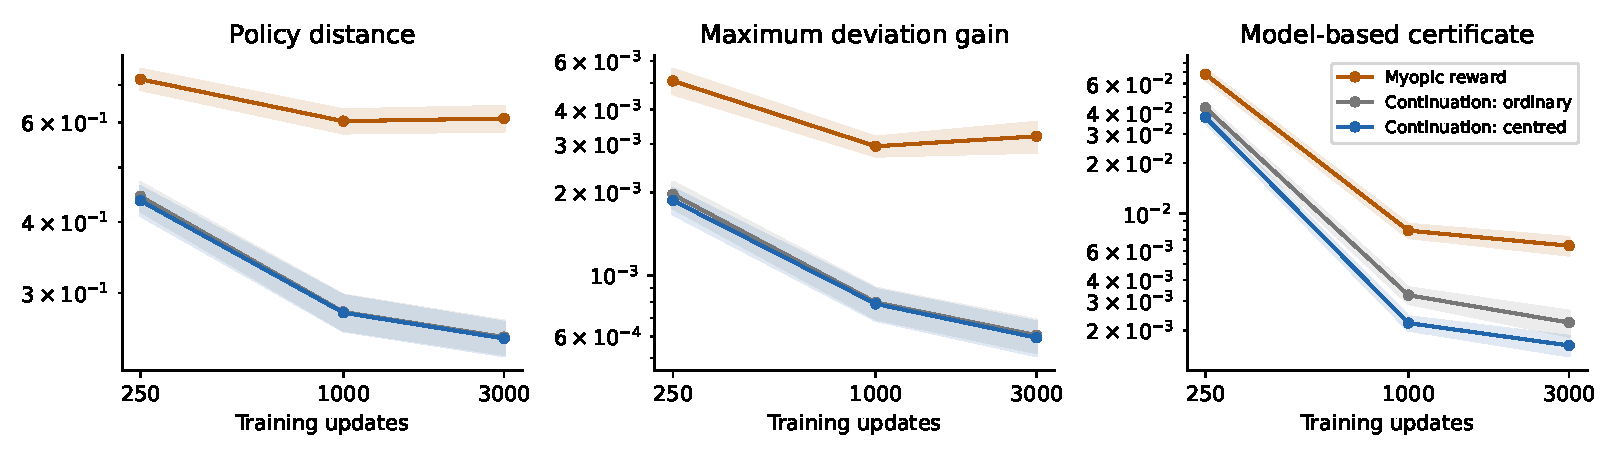
\includegraphics[width=\textwidth]{figures/rl_learning.pdf}
\caption{Shared neural actor--critic, twenty seeds and nine fixed markets. Means first average markets within seed; bands are descriptive mean $\pm1.96$ standard errors, not simultaneous intervals. The audit measures policy-relevant critic errors separately from observed performance.}
\Description{Three learning curves compare policy distance, true deviation gain and the model-based residual certificate for myopic, ordinary continuation and centred continuation learners.}
\label{fig:rl}
\end{figure*}

\PpoText\ The PPO result supports a reward intervention within a fixed optimiser; it does not establish algorithmic superiority over the recent equilibrium-RL frameworks in Section~2. Their continuous-time problems and model access differ from this benchmark.

The certificate catches a constructed false-convergence case: all critic-based action gradients are zero, yet the maximum true deviation gain is 0.10263. Its bound is 0.89674. Conversely, adding large state-constant critic offsets changes the certificate by less than $1.7\times10^{-15}$ across twenty saved cases. Random-policy tests compare deviation gains with independent terminal-moment calculations, including active action constraints. The vector projection inequality is also checked; these tests do not constitute a high-dimensional neural experiment.

\subsection{Auditing with independent samples}
Twenty fixed tabular policies in the $T=12,p=.8$ market receive 32,768 independent audit observations per time/state, or 786,432 each. Figure~\ref{fig:audit} compares bounds for each policy. Mean actual maximum deviation is 0.000902 and the exact-model bound is 0.001257. A Hoeffding-only observable bound averages 0.036141. Empirical Bernstein bounds with confidence-bounded transition mixing reduce this to 0.004911. Every policy is covered by each construction. Coverage in these twenty cases is a numerical check, not the source of the confidence guarantee.

The Bernstein and mixing refinements followed inspection of the initial loose bounds and are labelled a sequential extension. Each construction has its own 95\% simultaneous-over-states guarantee for a fixed policy; no joint 95\% guarantee across all policies or constructions is claimed. Large audit requirements and abstention when variance cannot be certified are substantive properties of the method.

\begin{figure}[t]
\centering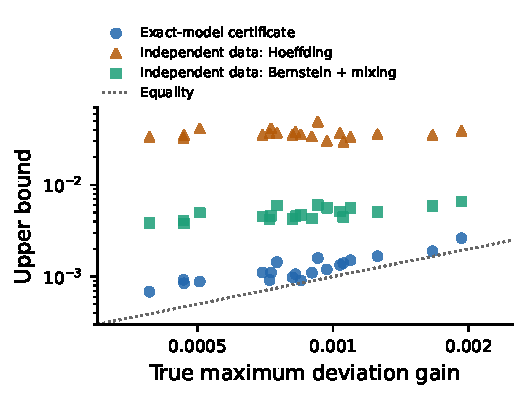
\includegraphics[width=\columnwidth]{figures/audit_bounds.pdf}
\caption{Can independent data certify a learned decision? Each point is one of twenty fixed policies. The refined data bound is tighter than Hoeffding alone but remains above the true gain. Each audit uses 786,432 observations; coverage is proved under the stated assumptions, not inferred from these points.}
\Description{Logarithmic scatter plot of true deviation gain against exact-model, Hoeffding and refined independent-data upper bounds. All displayed bounds exceed the actual gains.}
\label{fig:audit}
\end{figure}

\subsection{Financial inputs and implemented preferences}
Table~\ref{tab:historical} retains the historical published-formulation and covariance comparison. Its cross-estimator distances are changes in fitted models, not pure reward errors. The restricted Habibnia--Soltanzadeh comparator uses long-only unit-capital assetwise PnL, penalty 25 and cost multiplier $25/5$; SAC, shorting and lending are not replicated. Its objective depends on marginal downside payoffs and can prefer allocations different from mean--variance diversification.

\begin{table*}[t]
\centering
\caption{Ten industries, 1990--2025. Common-state distances and gaps use the fixed-diagonal MV reference; covariance rows change that reference model. Own-state paths determine realised metrics. Source entries are chronological; 2026 denotes this implementation for controls. Published formulations are adapted, not complete agent replications. Bold identifies our construction, not the best investment result.}
\label{tab:historical}
\begin{tabular}{@{}p{.235\textwidth}p{.25\textwidth}rrrr@{}}\toprule
Method & Source / role & \shortstack{Allocation\\distance} & \shortstack{Reference gap\\(bp)} & \shortstack{Excess\\Sharpe} & \shortstack{Realised MV\\(bp)}\\\midrule
Fitted MV reference & Markowitz (1952) & 0.00000 & 0.0000 & 0.570 & -8.497 \\
Minimum variance & Markowitz (1952) & 0.23843 & 9.0252 & 0.645 & 5.274 \\
MV, LW identity & Ledoit--Wolf (2004) & 0.00538 & 0.0055 & 0.572 & -8.442 \\
MV, LW correlation & Ledoit--Wolf (2004) & 0.02196 & 0.1158 & 0.547 & -11.917 \\
MV, market factor & Fan et al. (2008) & 0.05711 & 1.0487 & 0.585 & -4.738 \\
MV, three factors & Fan et al. (2008) & 0.04881 & 0.6407 & 0.555 & -8.532 \\
Equal weight & DeMiguel et al. (2009) & 0.43495 & 46.2626 & 0.622 & -11.893 \\
Raw second moment & Kolm--Ritter (2019) & 0.00843 & 0.0148 & 0.573 & -7.182 \\
MVPI adaptation & Zhang et al. (2021) & 0.00000 & 0.0000 & 0.570 & -8.497 \\
One MVPI step & Zhang et al. (2021) & 0.00014 & 0.0000 & 0.570 & -8.442 \\
Assetwise PnL, restricted & Habibnia--Soltanzadeh (2024) & 0.79645 & 40.2554 & 0.449 & -23.619 \\
Log minus variance & Jiang et al. (2025) & 0.01286 & 0.0287 & 0.572 & -7.123 \\
MV, sample covariance & Sample control (2026) & 0.01449 & 0.0356 & 0.555 & -10.114 \\
Log utility & Log-utility control (2026) & 0.54848 & 39.7855 & 0.344 & -133.295 \\
Unconstrained scalar & Analytical control (2026) & 0.00540 & 0.0043 & 0.568 & -8.882 \\
Risk-only calibration & Calibration ablation (2026) & 0.00510 & 0.0033 & 0.571 & -8.365 \\
\midrule
\textbf{Joint calibration (ours)} & \textbf{This study (2026)} & \textbf{0.00000} & \textbf{0.0000} & \textbf{0.570} & \textbf{-8.497} \\
\bottomrule\end{tabular}

\par\smallskip
\parbox{\textwidth}{\footnotesize Sources: Markowitz~\cite{markowitz1952}; Ledoit--Wolf~\cite{ledoit2004identity,ledoit2004correlation}; Fan et al.~\cite{fan2008}; DeMiguel et al.~\cite{demiguel2009}; Kolm--Ritter~\cite{kolm2019}; Zhang et al.~\cite{zhang2021}; Habibnia--Soltanzadeh~\cite{habibnia2024}; Jiang et al.~\cite{jiang2025}.}
\end{table*}

Across all eighteen covariance/universe cases, joint calibration has mean distance below $1.60\times10^{-7}$ from its own fitted reference. Raw distances range 0.00827--0.02249; transferring the unconstrained scalar formula worsens distance and fitted regret in all twelve larger-universe cases. One existing MVPI update initialised at holdings reduces mean distance by 97.8--98.6\%, without supplying the fitted optimum. These are calibration results, not a new MVPI algorithm.

Dimension increases $N/L $ from 0.083 to 0.250 and 0.408, with 65/495/1,274 distinct mean/covariance entries. The classifications also change the opportunity set, so this is not a causal experiment in dimension alone. DeMiguel et al.'s~\cite{demiguel2009} 3,000/6,000-month examples are model-dependent illustrations, not universal requirements. Simple controls and shrinkage remain essential.

Minimum variance has the highest realised MV among quadratic comparators in all eighteen cases, while joint calibration remains below raw. All fifteen cross-covariance target comparisons have paired 95\% intervals containing zero, including simultaneous path-bootstrap bands. Improved alignment therefore does not establish improved historical investment performance. In 2,160 known-covariance fitted problems, factor structure helps when its residual assumptions hold; misspecification can worsen population regret while leaving exact reward calibration intact. A separate fifty-state borrowing/shorting test gives joint distance $1.51\times10^{-7}$, versus 0.00997 when financing charges are not scaled. These results isolate estimation and cost mechanisms without claiming a replication of a crypto agent.

\begin{figure*}[t]
\centering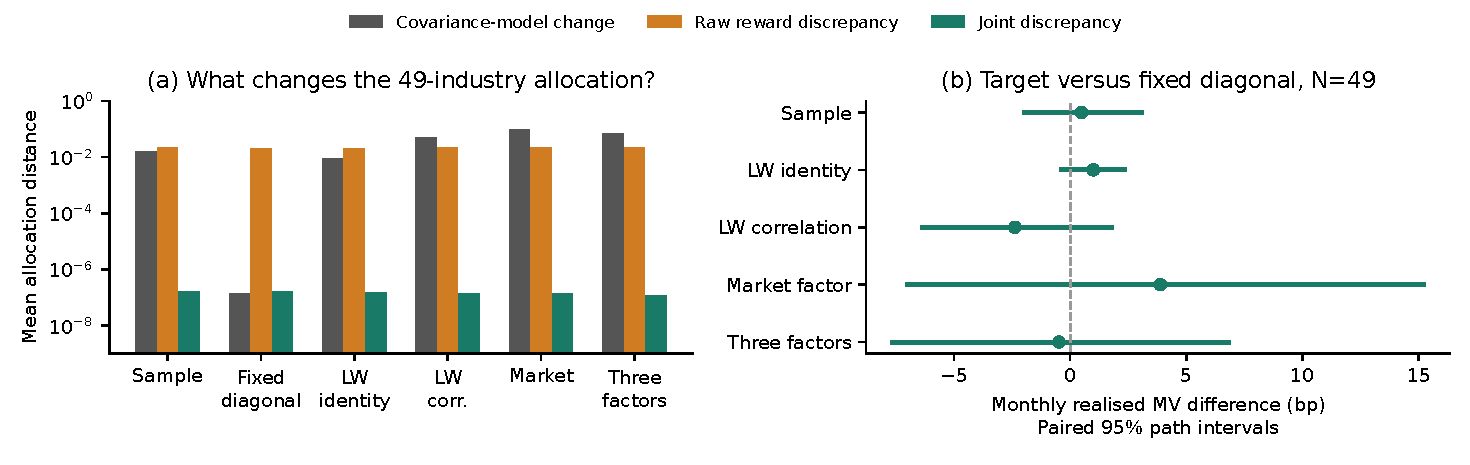
\includegraphics[width=\textwidth]{figures/covariance.pdf}
\caption{Covariance and reward interventions in the 49-industry universe. Within-model alignment and own-state realised performance answer different questions. The joint correction preserves the fitted preference; it does not identify the true covariance or dominate backtest returns.}
\Description{Historical covariance comparisons distinguish policy alignment within each model from realised investment performance.}
\label{fig:cov}
\end{figure*}

\section{Financial interpretation and validation}
An explanation of a financial agent should identify which decision changed and why. A covariance change alters estimated opportunities; a reward change alters preferences conditional on those opportunities; a critic or actor error alters how faithfully the learner implements the reward. Our historical common-state design and the residual certificate make these distinctions inspectable. In the 49-industry market-factor case, switching the covariance model changes the target by 0.09392 on average; within that model raw reward discrepancy is 0.02174 and joint discrepancy $1.36\times10^{-7}$. These numbers should not be combined into one undifferentiated error score.

The learning audit adds a further explanation: it identifies whether the agent could improve the stated conditional objective by changing an action. A state-constant critic error is harmless for the covariance hedge, while a state-dependent error can produce apparent actor convergence at a non-equilibrium policy. At constraints, feasible deviation gains avoid penalising a valid boundary optimum. This is financial decision interpretability and faithful evaluation, not an attribution explanation of hidden neural representations.

A validation record should state the mandate, information set, feasible actions, data vintage, uncertainty assumptions and acceptance tolerance. Theorem~\ref{th:audit} supports a quantitative acceptance rule when its assumptions hold; an infinite sample bound supports abstention when they do not provide enough information. Historical reward calibration can be checked without claiming to certify a true-market multiperiod equilibrium. Unknown regimes, market impact, wealth-dependent policies and transaction-cost states require a different continuation analysis.

Kolm and Ritter~\cite{kolm2025}, Exhibit~2 and pp.~90--91, distinguish reward specification, learning and decision quality. Our audit connects these stages and complements, rather than replaces, model-risk review. It takes the mandate as given, unlike inverse preference learning. For a tractable one-period allocation, direct optimisation remains appropriate. For a learned sequential policy, the useful output is not merely a Sharpe ranking but an explicit account of the decision error that remains.

\section{Conclusion}
Reward alignment can be audited after learning as well as before it. Under a finite exogenous-state market model, a residual certificate bounds the gain from departing from a learned policy relative to mean--variance equilibrium, ignores irrelevant critic offsets and accommodates convex constraints. Controlled actor--critic and PPO comparisons test the continuation correction without an oracle target. Historical covariance and cost experiments show why policy fidelity, estimation quality and realised returns must remain separate. The result is a reproducible financial validation method, with explicit conditions for when its certificate is informative.

\bibliographystyle{ACM-Reference-Format}
\bibliography{references}
\appendix
\section*{Appendix}
\section{Independent-data certificate}\label{app:data}
Fix a scalar policy $u $ and critic $c $ independently of audit data, and assume known support $|R|\le B $. At every $(t,z)$ obtain $N=2n $ independent conditional observations. Pair them and differentiate Eq.~\eqref{eq:paired}; each gradient sample has absolute bound
\[
 M_g=HB+2\varphi HB\spn(c_{t+1})+4\varphi H^2B^2|u|.
\]
The pair variable $(R_1-R_2)^2/2$ estimates conditional variance and lies in $[0,2B^2]$. Bellman targets have range at most $2HB|u|+\spn(c_{t+1})$. Hoeffding radii with failure probability $q=\alpha/(3TK)$ give a gradient upper norm, variance lower bound and residual intervals $[l_z,h_z]$. Then $\spn(e_t)\le\max_z h_z-\min_z l_z $; use $\rho_t\le1$ in Eq.~\eqref{eq:span}. Substitute these bounds in Eq.~\eqref{eq:audit}. The result covers all time/state cells with probability at least $1-\alpha $, conditional on training.

For a variable of known range width $W $ and sample size $n $, Maurer--Pontil~\cite{maurer2009}, Theorem~4, gives the two-sided radius
\[
 \sqrt{\frac{2\widehat V\log(4/q)}n}
 +\frac{7W\log(4/q)}{3(n-1)},
\]
where $\widehat V $ uses denominator $n-1$. Confidence intervals for each transition entry additionally give $\rho_t\le\min(1,\widehat\rho_t+K\eta)$, where $\eta $ bounds each entry error. Include $TK^2$ additional events in the union bound. The construction returns infinity if any variance lower bound is nonpositive. Adaptive policy selection on the audit set, dependent observations or unknown support require additional analysis; none is assumed here. The scalar implementation bounds unrestricted deviations, which also upper-bound constrained ones.

\section{Raw-reward discrepancy}\label{app:raw}
For constant independent moments with $m\ne0$, the quadratic Bellman solution has $u_t=\alpha_tx+\beta_t $, with terminal $p_T=q_T=0$ and $g_t=\kappa(s-1)-sp_{t+1}$:
\begin{align*}
\alpha_t&=-dg_t/(\kappa-p_{t+1}),\\
\beta_t&=d(1+q_{t+1})/[2(\kappa-p_{t+1})],\\
p_t&=[\kappa p_{t+1}-(1-\nu)g_t^2]/(\kappa-p_{t+1}),\\
1+q_t&=(1+q_{t+1})[s-\nu g_t/(\kappa-p_{t+1})].
\end{align*}
Induction gives $p_t\le0$, hence global concave action maximisation. Put $e=s-1$ and $h=(2\kappa)^{-1}$. Because $p_t/\kappa,q_t $ are independent of $\kappa $, the wealth recursion is affine in $h $ and $D^2$ is exactly quadratic in $h $, analytic near $e=0$. At zero it is $T\|d\|^2(h-b)^2$, so its positive minimiser is analytic nearby.

Writing $\kappa=\varphi(1-\nu)(1+we)$, the leading action error is $de[-X_t+b((T-t-1)(2-\nu)-w)]$. At $e=0$, mean wealth is $x_0+t\nu b $ and variance $tb^2\nu(1-\nu)$. Minimisation gives $w=(T-1)(1-\nu)-x_0/b $; summing centred mean squares $b^2(T-1-2t)^2$ and wealth variances yields Eq.~\eqref{eq:raw}. This is a fixed-horizon expansion, not a uniform joint limit. For $s\ne1$, exact matching is impossible: matching initially creates positive subsequent wealth variance, whereas the final raw policy has nonzero wealth slope $-d(s-1)$ and equilibrium is constant.

\section{Reproduction and numerical checks}\label{app:repro}
The fixed conditional-sample generators use seeds 0--19; neural seeds also control weights and minibatches. PPO uses seeds 0--9, eight vector environments and a deterministic deployed-policy evaluation; both arms have identical data access and refresh frequency. Its continuation function is fitted from the current policy and training outcomes, not the analytic reference. The neural five-seed pilot, twenty-seed extension and later PPO experiment are retained separately. Paired bootstrap intervals use 10,000 resamples of seed averages; all final-budget runs are retained.

Historical identity shrinkage uses centred $Z $, $S_0=Z^\top Z/L $ and target $\operatorname{tr}(S_0)I/N $, with intensity from the empirical fourth moment; final covariance is converted to denominator $L-1$. Constant-correlation shrinkage uses the inspected Ledoit--Wolf working-paper plug-in formulas. Factor models use intercept OLS, market/SMB/HML and diagonal residual variances with denominator $L-K-1$. This finite-sample convention adapts Fan et al.~\cite{fan2008}. Missing and duplicate months are rejected. Holdings drift with gross asset returns; costs are charged separately at the stated first-order rate.

Historical uncertainty uses 1,000 shared circular twelve-month blocks, seed 8128, conditional on realised strategy paths; simultaneous covariance bands use the maximum centred deviation across fifteen comparisons. Quadratic optimisation is checked independently by a first-order linear-programme certificate in original objective units, with accepted gap at most $2\times10^{-7}$. Reconstruction verifies 58,320 historical decisions, 2,160 known-covariance fitted problems and 144 anchor checks. RL tests independently evaluate terminal moments, gradient/covariance identities, critic offsets, active boundaries and audit support. The source, fixed protocols, per-seed policies and machine-readable outputs reproduce the reported numerical checks. The claims and proofs are self-contained.
\end{document}
